\documentclass[twocolumn]{article}
\usepackage[utf8]{inputenc}
\usepackage{changepage}
\usepackage{graphicx}
\usepackage{amsmath}
\usepackage{amssymb}
\usepackage{amsthm}
\usepackage{mathtools}
\usepackage{float}
\usepackage[siunitx]{circuitikz}
\usepackage{tikz}
\usepackage{pgfplots}
\usepackage[colorlinks=true, linkcolor=black, citecolor=black, urlcolor=blue]{hyperref}
\usepackage{listings}
\pgfplotsset{width=10cm,compat=1.9}
\usetikzlibrary{positioning, arrows.meta}
\usepackage[a4paper, total={6in, 10in}]{geometry}
\bibliographystyle{ieeetr}

\title{\textbf{PROJECT VOICE - Galvanic Skin Response Sensors}}
\author{\textbf{Julian Edelman}}

\begin{document}

\maketitle

\section{Galvanic Skin Response Overview and Relevance to the Project}

Galvanic Skin Response (GSR) sensors, also known as electrodermal activity sensors, are valuable tools in understanding emotional and cognitive responses in individuals. These sensors measure changes in skin conductance, which varies with moisture level due to sweat gland activity. This is particularly influenced by various factors, including emotional arousal, stress, or anxiety. Understanding these variations is critical, especially in contexts where individuals may face communication barriers.

This method can serve as a means to assess responses of non-verbal individuals to various stimuli, thereby elucidating their cognitive engagement despite their challenges in verbal expression. For instance, individuals with autism or speech impairments may not articulate their feelings yet still exhibit emotional responses visible through GSR measurements.

\section{Technical - How it Works}

\subsection{How GSR Works}
Galvanic Skin Response (GSR) is a physiological reaction that indicates changes in skin conductance related to emotional arousal and autonomic nervous system activity. The skin, the largest organ in the human body, consists of three primary layers: the epidermis, which serves as a protective barrier; the dermis, which provides cushioning and support; and the hypodermis, which anchors the skin to muscles and bones. The skin contains approximately three million sweat glands, which become activated during emotional experiences, leading to an increase in moisture on the skin's surface. This moisture alters the balance of ions, resulting in changes in electrical conductivity, which can be measured as GSR.\cite{imotionsGalvanicSkin}

    \begin{figure}[H]
    \centering
    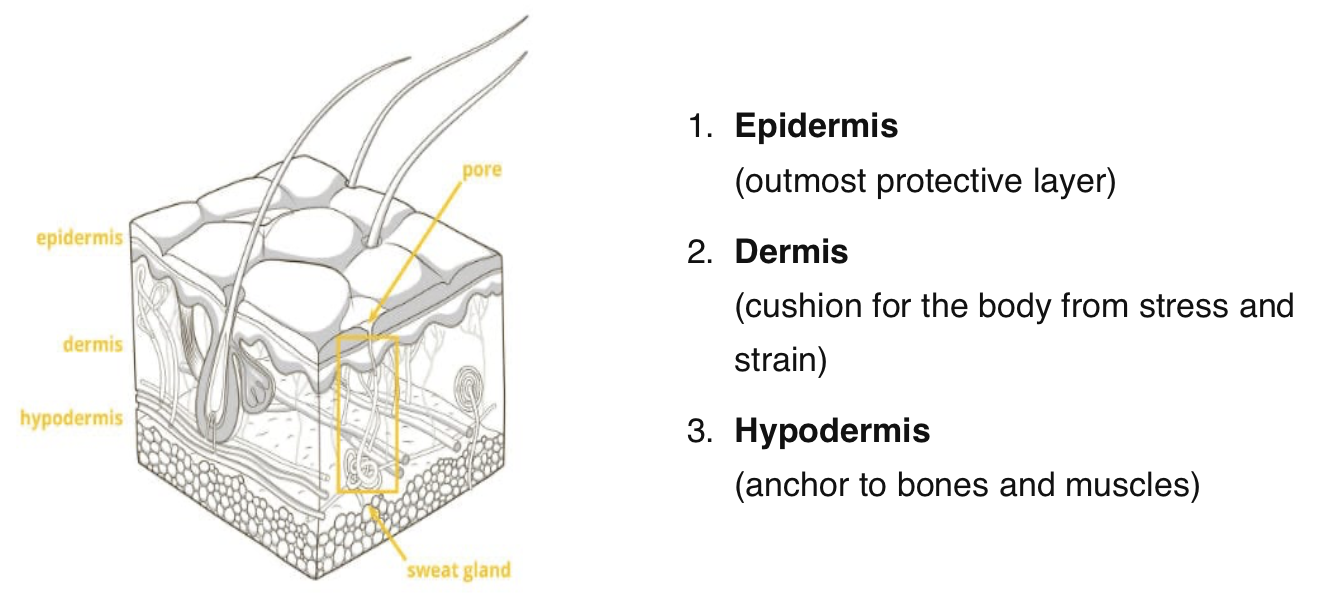
\includegraphics[width=\linewidth]{skin_perception.png}
    \caption{Skin cell from \cite{imotionsGalvanicSkin}}
    \label{fig:NR}
    \end{figure}

Sweat production, particularly in the hands and feet during emotional arousal, is an involuntary process controlled by the autonomic nervous system. This system consists of two branches: the sympathetic nervous system, which triggers rapid responses like "fight or flight," and the parasympathetic nervous system, which manages slower, restorative processes. Enhanced sympathetic activity leads to observable signs of arousal, such as increased heart rate, blood pressure, and sweating. By measuring GSR, one can gain insights into emotional states, underscoring the connection between physiological responses and psychological experiences.\cite{imotionsGalvanicSkin}

\section{GSR and Other Biometrics}

The effectiveness of GSR can be further enhanced when combined with other biometric measures. "For instance, integrating GSR data with signals from Electroencephalogram (EEG) or Electromyography (EMG) can provide a more comprehensive understanding of an individual's emotional and cognitive state."\cite{Wan_Wang_Wang_Tang_Liu_2024} Such multimodal approaches enable researchers to analyze emotional responses through different angles, leading to robust classification algorithms and improving insight into the interplay between various physiological signals.

\subsection{Physiological Responses to Mental Tasks - Harvard Study}

This study aimed to investigate whether pupil dilation is uniquely sensitive to mental effort or if similar results can be obtained with other autonomic functions when time-locked to paced mental activity. The experiment involved ten college students performing a digit transformation task at three levels of difficulty while their pupil size, skin resistance, and heart rate were measured. Participants were instructed to add 0, 1, or 3 to each of four serially presented digits and read out the transformed series after a 2-second pause. The procedure was paced by 1-second pulses, and measurements were time-locked to the task performance.\cite{article}

    \begin{figure}[H]
    \centering
    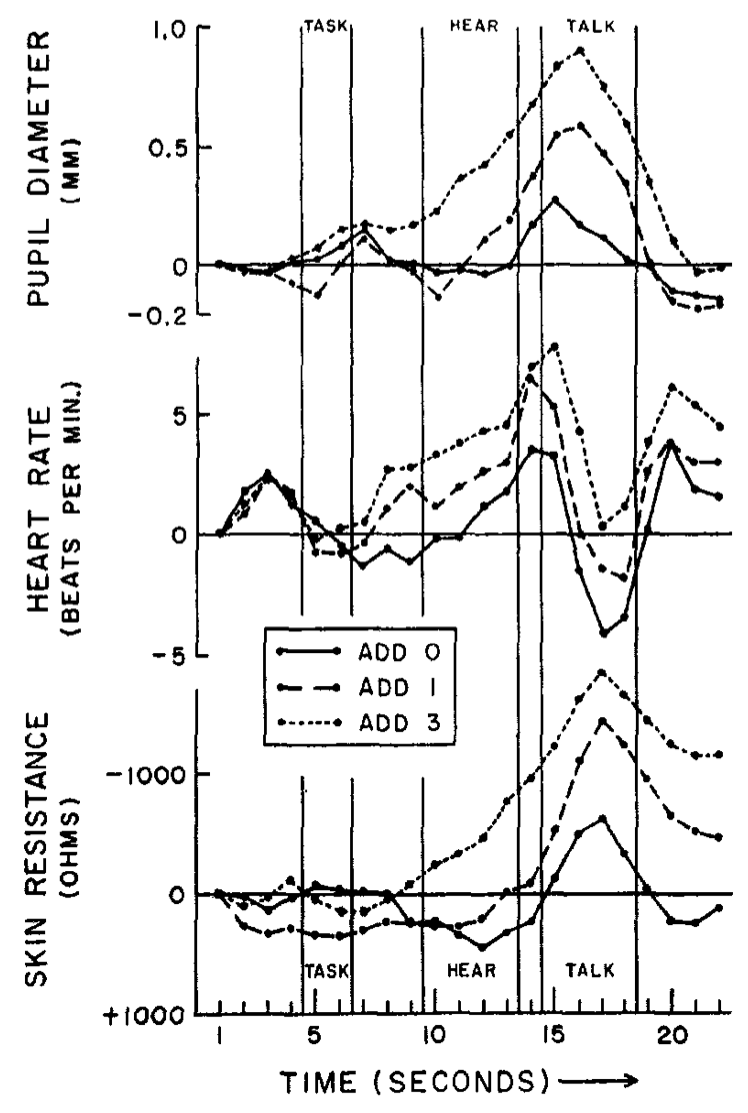
\includegraphics[width=\linewidth]{harvard_study.png}
    \caption{Second-by-second autonomic changes
    during digit transformation task from \cite{imotionsGalvanicSkin}}
    \label{fig:NR}
    \end{figure}

The study found that skin resistance, along with pupil size and heart rate, showed a sympathetic-like increase in activity during the input and processing of information, followed by a decrease in the report phase. The degree to which response magnitude was ordered as a function of task difficulty was assessed using Kendall's coefficient of concordance (W). For skin resistance, the W value was $0.48 (p < 0.02)$, indicating a significant correlation between task difficulty and skin resistance changes. This correlation was similar to that observed for pupil dilation $(W = 0.79, p < 0.001)$ and heart rate $(W = 0.25, p < 0.09)$, although the heart rate results were only marginally significant. The skin resistance response was particularly sensitive to the transformation effect $(W = 0.48, p < 0.02)$ rather than the instruction effect. The time course of response in all three channels was generally quite similar, but skin resistance showed a slower response compared to pupil dilation and heart rate, with maximal change occurring late in the report phase. Overall, the study demonstrated that precise tracking of changing mental effort was not unique to pupillary response, and skin resistance provided generally redundant information along with other autonomic measures.\cite{article}

\subsection{Implications of Harvard Study}

By integrating GSR data with metrics such as heart rate variability or electrodermal activity, researchers can develop a more comprehensive understanding of an individual's psychological state. This multi-faceted approach not only enhances the accuracy of emotional state assessments but also provides a more robust framework for interpreting GSR data in the context of broader physiological responses.\cite{Abdel-Latif_Rashid_Askari_Park_Sharp_Quinn_Cinar_2023}

The applications of GSR extend beyond traditional laboratory settings, finding increasing relevance in various fields such as consumer research, human-computer interaction, and mental health monitoring. In marketing and product development, GSR data can provide valuable insights into consumer emotional responses to advertisements, product designs, or user interfaces, helping companies optimize their offerings for better engagement. In the realm of mental health, continuous GSR monitoring through wearable devices shows promise for early detection of stress and anxiety disorders, potentially enabling timely interventions. Furthermore, the integration of GSR data with machine learning algorithms is opening new avenues for automated emotion recognition systems, which could have far-reaching implications for personalized technology and adaptive user experiences. As the technology continues to evolve, the potential applications of GSR in both research and practical settings are likely to expand, offering new ways to understand and respond to human emotional states.
\cite{Chen_Zeng_Chen_Cai_Wang_Wang_Zhang_Li_Yan_Siok_et_al._2024}

\section{Reading GSR Data}

Interpreting GSR data involves a systematic method encompassing data collection, preprocessing, and analysis. Initially, GSR data is gathered using sensors placed on the skin, typically on fingers or palms. The collected raw data is subject to preprocessing steps such as filtering out noise and normalizing signals to enhance signal integrity. These preprocessing steps ensure that the data reflects true physiological responses without being skewed by external factors or artifacts.

Once the data is prepared, analysis methodologies come into play. Researchers may employ statistical analysis to evaluate relationships between skin conductance levels and emotional stimuli, exploring correlations between GSR readings and reported emotional states. Machine learning algorithms may also be utilized to classify emotional states based on gathered data, improving the ability to predict and understand user emotions in real time. Through these processes, GSR can provide detailed emotional landscapes, enhancing both research outcomes and practical applications.

\subsection{GSR Signal Components}
GSR data "consists of two main components: tonic and phasic responses. Understanding these components is crucial for accurately interpreting GSR signals and their implications for emotional and cognitive states."\cite{Hernando-Gallego_Luengo_Artés-Rodríguez_2018}

\subsection{Tonic Component: Skin Conductance Level (SCL)}
The tonic component, referred to as Skin Conductance Level (SCL), represents the slow-changing baseline level of electrical conductivity of the skin. SCL reflects general changes in autonomic arousal and can vary due to factors such as hydration, skin dryness, and overall psychological state. Typically, SCL is measured in microsiemens ($\mu$S) and ranges from 2 to 20 $\mu$S, although individual differences can be significant.\cite{Hernando-Gallego_Luengo_Artés-Rodríguez_2018}

\subsection{Phasic Component: Skin Conductance Response (SCR)}
The phasic component, known as Skin Conductance Response (SCR), represents rapid changes in skin conductance in response to specific stimuli or events. SCRs are characterized by a sudden increase in conductance followed by a gradual return to baseline.\cite{Hernando-Gallego_Luengo_Artés-Rodríguez_2018}

Key features of SCRs include:

\begin{enumerate}
    \item Amplitude: The magnitude of the response, typically measured from the onset to the peak of the SCR.\cite{Hernando-Gallego_Luengo_Artés-Rodríguez_2018}
    \item Latency: The time between stimulus onset and the beginning of the SCR.\cite{Hernando-Gallego_Luengo_Artés-Rodríguez_2018}
    \item Rise Time: The time taken for the response to reach its peak.\cite{Hernando-Gallego_Luengo_Artés-Rodríguez_2018}
    \item Recovery Time: The time taken for the response to return to baseline.\cite{Hernando-Gallego_Luengo_Artés-Rodríguez_2018}
\end{enumerate}

\subsection{Quantifying GSR Signals}
To quantify GSR signals, researchers often use mathematical models to separate the tonic and phasic components. One common approach is the use of deconvolution techniques. The observed GSR signal $y(t)$ can be modeled as:

\[
y(t) = r(t) * \delta(t) + n(t)
\]

Where $r(t)$ is the impulse response function (IRF), $\delta(t)$ represents the sudomotor nerve activity, and $n(t)$ is noise.

\subsection{Interpreting GSR Data}
When interpreting GSR data, it's essential to consider both the tonic and phasic components. An increase in SCL generally indicates heightened arousal or stress, while frequent and large SCRs suggest higher emotional reactivity or cognitive load. However, it's crucial to interpret these signals in context, considering factors such as individual differences, environmental conditions, and the nature of the stimuli.\cite{Hernando-Gallego_Luengo_Artés-Rodríguez_2018}

\subsection{Advanced Analysis Techniques}
Modern GSR analysis often employs advanced signal processing techniques to extract more nuanced information. For instance, researchers may use continuous decomposition analysis (CDA) to separate overlapping SCRs and estimate the underlying sudomotor nerve activity. Machine learning algorithms are also increasingly used to classify emotional states based on GSR patterns, often in combination with other physiological signals.

\subsection{Practical Considerations}
When collecting and analyzing GSR data, several practical considerations are important:

\begin{enumerate}
    \item Sensor placement: Typically, GSR sensors are placed on the palmar surface of fingers or the sole of the foot, where sweat gland density is high.\cite{Hernando-Gallego_Luengo_Artés-Rodríguez_2018}
    \item Signal filtering: Raw GSR signals often require filtering to remove noise and artifacts.\cite{Hernando-Gallego_Luengo_Artés-Rodríguez_2018}
    \item Baseline correction: Establishing a proper baseline is crucial for accurate interpretation of changes in GSR.\cite{Hernando-Gallego_Luengo_Artés-Rodríguez_2018}
\end{enumerate}

By carefully considering these factors and employing appropriate analysis techniques, researchers can extract valuable insights from GSR data, providing a window into the complex interplay between physiological responses and psychological states.\cite{Hernando-Gallego_Luengo_Artés-Rodríguez_2018}

\section{Conclusion}

In conclusion, GSR sensors present a powerful tool for emotion and attention classification, which could be used in aiding the understanding of non verbal communication. Their non-invasive nature, ease of implementation, and direct measurement of arousal enhance their utility in understanding complex emotional states. As research continues to evolve, integrating GSR with other physiological measures and standardizing methodological approaches will strengthen the capabilities of emotion recognition technologies. This integration has the potential to create more nuanced systems capable of responding dynamically to human emotional experiences.

\bibliography{citations}

\end{document}